\documentclass[11pt]{article}
\usepackage[T1]{fontenc}
\usepackage[margin=1in]{geometry}
\usepackage{amsmath,booktabs,graphicx,float,longtable,hyperref}
\title{Experiment 05 --- Spectral Lag and Latent Boundary Corrections}
\author{Two-Layer CTMC experimental framework}
\date{DEVELOPMENT RESULTS --- NOT FINAL}
\begin{document}
\maketitle
\begin{center}\fbox{\textbf{DEVELOPMENT RESULTS --- NOT FINAL}}\end{center}

\begin{abstract}
This experiment tests two candidate aggregate-descriptor corrections to premature
inter-community leakage in MicroMacro simulation.  A spectral lag delays source
contagiousness, while a latent-boundary state relaxes toward aggregate prevalence.
Full Micro is the reference and all five variants share the network and initial
condition within a replication.  Inference uses the replication as the independent
unit and distinguishes completed-only Wasserstein metrics from censoring-aware
all-run RMST metrics.  The present document reports the validation stage.
These development estimates are diagnostic and are not final scientific conclusions.
\end{abstract}

\section{Research question}
Can spectral lag, latent-boundary relaxation, or their combination reduce sparse
chain-of-cliques terminal-arrival bias without knowing bridge-node identities?

\section{Motivation}
Section 3.7 of \emph{Notes on Micro--Macro Epidemic Networks} reports premature
leakage in the sparse benchmark. Experiment 01 separated hazard and placement
effects but left bridge-specific error. The corrections tested here are
\emph{candidate corrections proposed within the experimental framework, motivated
by spectral epidemic-threshold bounds}; they are not attributed to the article.

\section{Experimental design}
The five paired variants are V0 Full Micro, V1 production aggregate MicroMacro,
V2 lag-shifted MicroMacro, V3 latent-boundary MicroMacro, and V4 combined.
The baseline has $L=10$, $n=100$, $k=5$, mean internal degree approximately 6,
$\beta_{in}=\beta_{out}=0.003$, $\gamma=0$, $\tau_{micro}=1$, and
$T_{end}=4000$. Mini-sweeps vary $k\in\{1,5,10\}$ and
$d\in\{4,6,10\}$ without taking a Cartesian product. Network and initialization
streams are shared within replication; event streams are variant-specific.

\section{Mathematical definitions}
For community $i$, $N_i$ is its size, $i_i(t)$ its infected count,
$\bar i_i(t)=i_i(t)/N_i$, and $\bar s_j(t)$ is normalized susceptibility.
The reference macro hazard is
\[\lambda^{ref}_{ij}(t)=\beta_{out}W_{ij}\bar i_i(t)\bar s_j(t).\]
The lag is
\[\tau_{find}(i)=\frac{\ln N_i}{\beta_{in}(\lambda_1(G_i)-1)},\qquad
  \bar i_i^{lag}(t)=\bar i_i(\max(0,t-\tau_{find}(i))),\]
and $\lambda^A_{ij}=\beta_{out}W_{ij}\bar i_i^{lag}\bar s_j$.
The latent rate and analytical synchronization update are
\[\kappa(i)=\frac{\beta_{in}(\lambda_1(G_i)-1)}{\ell(G_i)},\qquad
\bar i_i^B(t+\tau)=\bar i_i^B(t)+(1-e^{-\kappa(i)\tau})
  (\bar i_i(t)-\bar i_i^B(t)),\]
with $\bar i_i^B(0)=0$ and $\lambda^B_{ij}=\beta_{out}W_{ij}\bar i_i^B\bar s_j$.
V4 applies the same latent update to $\bar i_i^{lag}$. If $\lambda_1\le1$ or
$\ell$ is undefined, corrected outgoing hazard is zero and the descriptors are
flagged degenerate. Arrival definitions are $T_i=\inf\{t:i_i(t)>0\}$,
$T_{last}=T_{L-1}$, and $\Delta T_i=T_{i+1}-T_i$; censored values equal
$T_{end}$ with a separate observation flag.

\section{Parameters}
Each configured scenario uses a connected fixed-edge-count Erd\H{o}s--R\'enyi
community, uniform susceptible import placement, and one uniformly selected seed
in community zero. Graph descriptors are computed once before simulation.

\section{Implementation details}
Adjacency spectral radius is computed by shifted power iteration to tolerance
$10^{-6}$ with at most 1000 iterations and a residual-norm convergence check.
Mean shortest-path length is computed on the unweighted local graph. Lag history
uses fixed synchronization points and linear interpolation. The latent ODE uses
the analytical exponential update, not Euler integration. No descriptor fallback
is permitted. Outputs retain deterministic stream metadata and per-replication
graph checksums. Additional diagnostics have distinct purposes: integrated hazard
suppression measures how strongly each correction changes V1 exposure; synchronized
correlation between $\bar i_i$ and the latent state checks relaxation semantics; and
V0 time-to-first-boundary versus $\tau_{find}$ assesses the spectral lag as a
descriptor without feeding bridge identity into a corrected variant.

\section{Sanity checks}
\begin{table}[H]\centering
\caption{Recorded stage gates and actual diagnostic values.}
\begin{tabular}{p{.24\linewidth}p{.58\linewidth}p{.12\linewidth}}\toprule Gate & Value & Status \\\midrule
pairing & groups=100; failures=0 & passed \\ 
snapshot\_parquet\_metadata & \{"failures": 0, "files\_checked": 500\} & passed \\ 
snapshot\_raw\_sha256 & \{"failures": 0, "files\_checked": 500\} & passed \\ 
source\_writer\_isolated & snapshot contains checkpoint summaries only; active raw/checkpoints are not modified & passed \\ 
\bottomrule\end{tabular}\end{table}
Interpretation below is conditional on the formula, reproducibility, pairing,
reference, schema, and production-immutability gates recorded in the manifest.

\section{Results tables}
Table 1 labels $W_1$ as completed-only and RMST/completion as all-run metrics.
\begin{longtable}{llrrrr}
\toprule
Scenario & Variant & rel. $W_1$ & $\Delta$RMST [95\% CI] & Completion & Status \\
\midrule
\endfirsthead
\toprule
Scenario & Variant & rel. $W_1$ & $\Delta$RMST [95\% CI] & Completion & Status \\
\midrule
\endhead
baseline & Full Micro & 0 & 0 [0, 0] & 0.99 & ok \\
baseline & Baseline MicroMacro & 0.06939 & 200.6 [98.25, 307.7] & 0.98 & ok \\
baseline & Lag & NA & 1071 [995.9, 1152] & 0 & no\_completed\_arrivals \\
baseline & Latent boundary & 0.2421 & 905.8 [807.4, 989.9] & 0.44 & ok \\
baseline & Lag + latent & NA & 1071 [991, 1146] & 0 & no\_completed\_arrivals \\
\bottomrule
\end{longtable}


\section{Figures}
\begin{figure}[H]\centering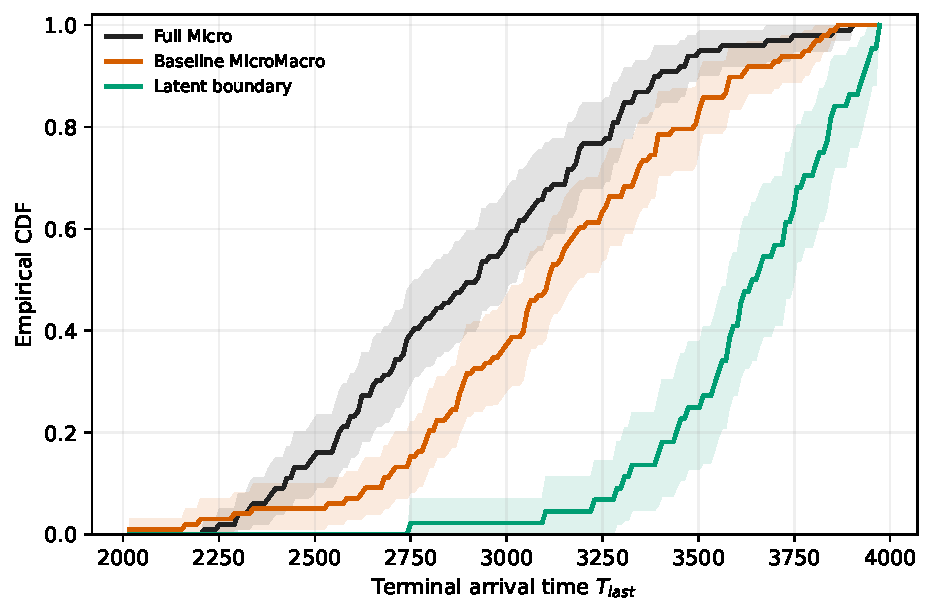
\includegraphics[width=.78\linewidth]{figures/figure_1.pdf}
\caption{Baseline empirical CDF of completed terminal arrivals. Bands are pointwise
95\% replication-bootstrap intervals; the statistical unit is a replication.}\end{figure}
\begin{figure}[H]\centering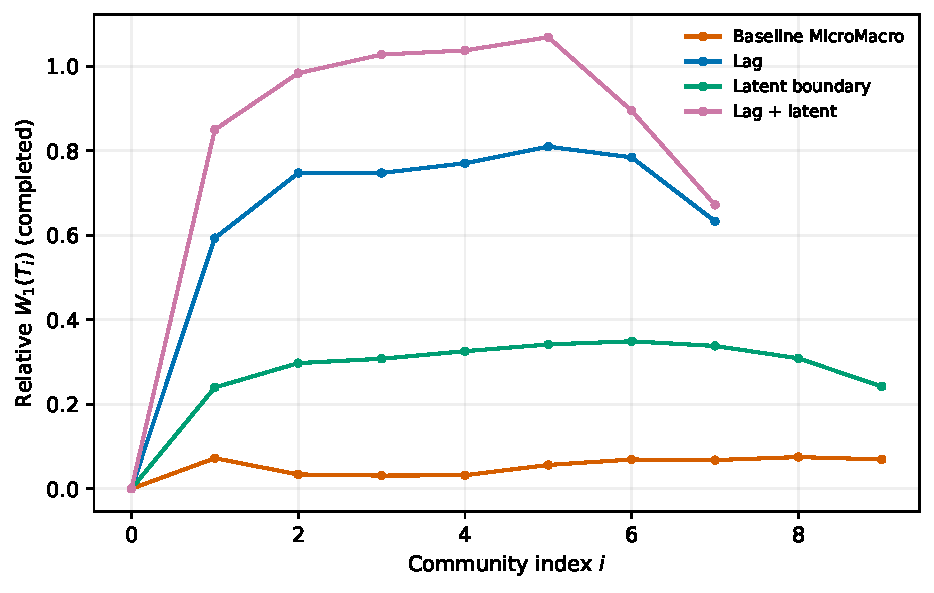
\includegraphics[width=.78\linewidth]{figures/figure_2.pdf}
\caption{Layer-wise completed-only relative $W_1(T_i)$ against V0. The statistical
unit is a replication.}\end{figure}
\begin{figure}[H]\centering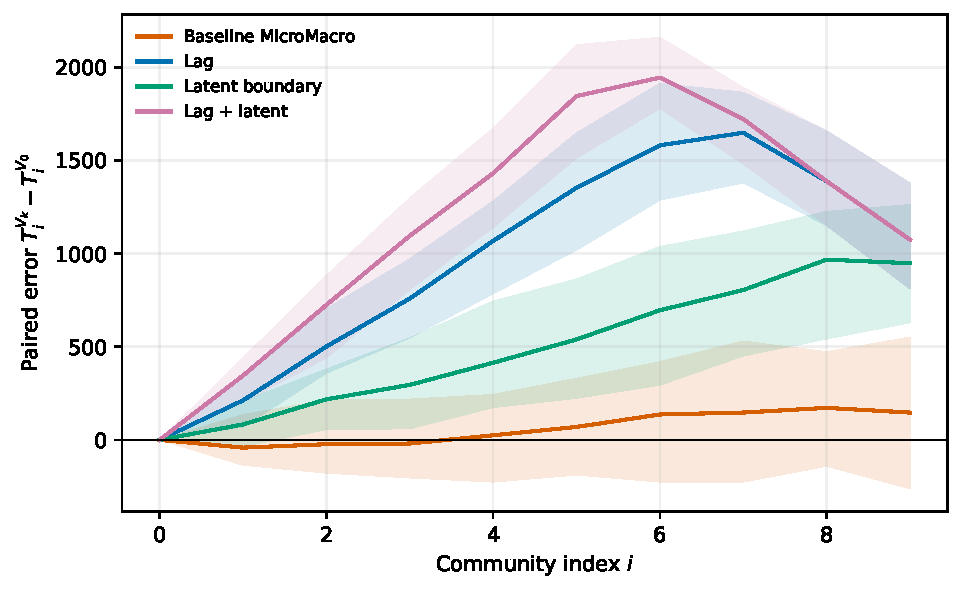
\includegraphics[width=.78\linewidth]{figures/figure_3.pdf}
\caption{Paired cumulative arrival error (variant minus V0), median and IQR over
replications; censored arrivals retain the common horizon.}\end{figure}
\begin{figure}[H]\centering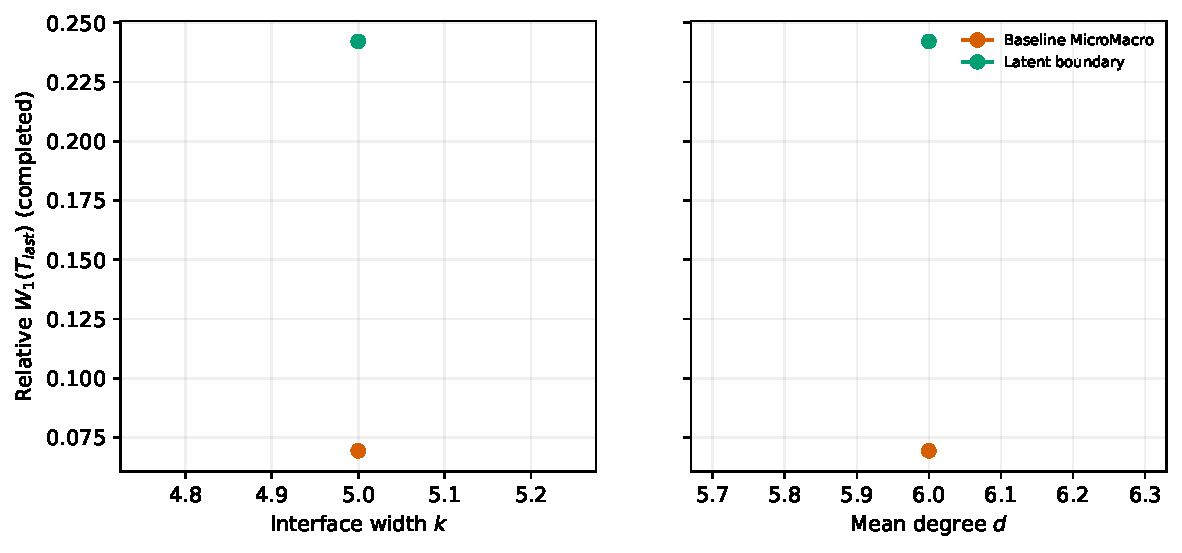
\includegraphics[width=.88\linewidth]{figures/figure_4.pdf}
\caption{Completed-only terminal relative $W_1$ across the interface-width and
density mini-sweeps. Baseline supplies the shared $k=5,d=6$ point.}\end{figure}

\section{Uncertainty analysis}
All confidence intervals use 1000 paired bootstrap resamples of
replication IDs. Event rows are never bootstrap units. $W_1$ compares completed
terminal-arrival distributions and is normalized by the V0 completed mean.
$\Delta$RMST is variant minus V0 using all horizon-restricted runs. Equivalence
requires the entire $\Delta$RMST interval to lie within
$\pm0.05\,\mathrm{mean}(T_{last}^{V0})$.

\section{Scientific interpretation}
H1 is assessed by V2 versus V1, H2 by V3 versus V1, and their joint behavior by
V4. The replication-level factorial interaction $V4-V2-V3+V1$ on restricted
terminal arrival is -705.2 (95\% CI -799.8 to -613.3). Claims of improvement require both passed
gates and the reported uncertainty intervals; an interval containing zero alone
is not evidence of equivalence. In the baseline validation sample, V1 completed in 98\% of runs with relative completed-only $W_1=0.06939$. H1 (V2) and H1+H2 (V4) each had zero terminal completions, so their terminal $W_1$ values are undefined; their all-run $\Delta$RMST values were 1071 and 1071. H2 (V3) completed in 44\% of runs, with relative completed-only $W_1=0.2421$ and all-run $\Delta\mathrm{RMST}=905.8$. Thus none of the literal corrections improved the validation outcome over V1; this development sample does not confirm H1, H2, or monotone additivity.

\section{What the experiment can identify}
It can estimate relative bias reduction in the sparse baseline, distinguish H1
from H2 within the factorial cells, assess their interaction, and describe limited
scaling across the specified $d$ and $k$ values.

\section{What the experiment cannot identify}
It cannot identify recovery effects, synchronization-interval effects, placement
effects, generalization beyond connected ER communities, or computational speedup.
Runtime is an implementation diagnostic only.

\section{Limitations}
Lag may interact with midpoint hazard integration, and latent relaxation may
interact with the exponential-clock residual update. The spectral formula is a
candidate scaling law over a small descriptor range. Completed-only Wasserstein
statistics condition on arrival and therefore must be read beside completion and
all-run RMST.

\section{Unresolved questions}
The current design does not determine whether any remaining discrepancy is caused
by synchronization timing, placement, or non-ER boundary geometry.

\section{Recommended next experiment}
No recommendation is made outside the staged Experiment 05 evidence. Any follow-up
specified here after validation must preserve pairing and separately vary only one
previously fixed mechanism.

\section{Exact reproduction commands}
\begin{verbatim}
python -m two_layer_ctmc.experiments.experiment_05_spectral_corrections.cli \
  --stage smoke --scenario baseline --replications 5 --master-seed 270000
python -m two_layer_ctmc.experiments.experiment_05_spectral_corrections.cli \
  --stage validation --scenario all --replications 20 --resume --master-seed 270000
# Run only after explicit approval:
python -m two_layer_ctmc.experiments.experiment_05_spectral_corrections.cli \
  --stage final --scenario all --replications 100 --resume \
  --validation-approved --master-seed 270000
\end{verbatim}
\end{document}
